\section{Discussion \& Limitations}
\label{sec:discussion}

\subsection{Insulation from Calibration Poisoning}
The original pure causal framework (v1) was highly sensitive to training contamination. Leakage of attack windows into the calibration set inflated the risk score baseline distribution, preventing subsequent test alerts. In our Causal Behavioral State Reasoning framework, the use of a partially labeled validation set helps insulate the system:
\begin{itemize}
\item The Behavioral Pattern Reasoner (BPR) is trained on validation state coordinates and labels, allowing it to explicitly learn the decision boundary between benign noise and attack patterns.
\item The stacked fusion meta-operator dynamically adjusts operator weights, mitigating the impact of an inflated calibration queue on the overall threat risk.
\end{itemize}
While validation labeling introduces a small manual overhead (transitioning the framework to a semi-supervised setup), it represents a favorable security trade-off by hardening the system against calibration poisoning.

\subsection{Causal Discovery Overhead \& Operational Latency}
RobustParCorr causal discovery on BETH ($d = 882$ features, $T = 360$ training windows) requires 7,842 seconds ($\approx$2.18 hours) on a standard CPU. This is a \textbf{one-time offline or asynchronous background process} that runs during system commissioning or periodically during idle hours. Figure~\ref{fig:scalability_curve} illustrates the scalability trade-off. Once SCM coefficients are stored, online behavioral state projection and multi-perspective reasoning runs in \textbf{1.13--1.21\,ms per window} (Table~\ref{tab:runtime_hybrid}), easily supporting high-throughput enterprise streams.

\begin{figure}[htbp]
\centerline{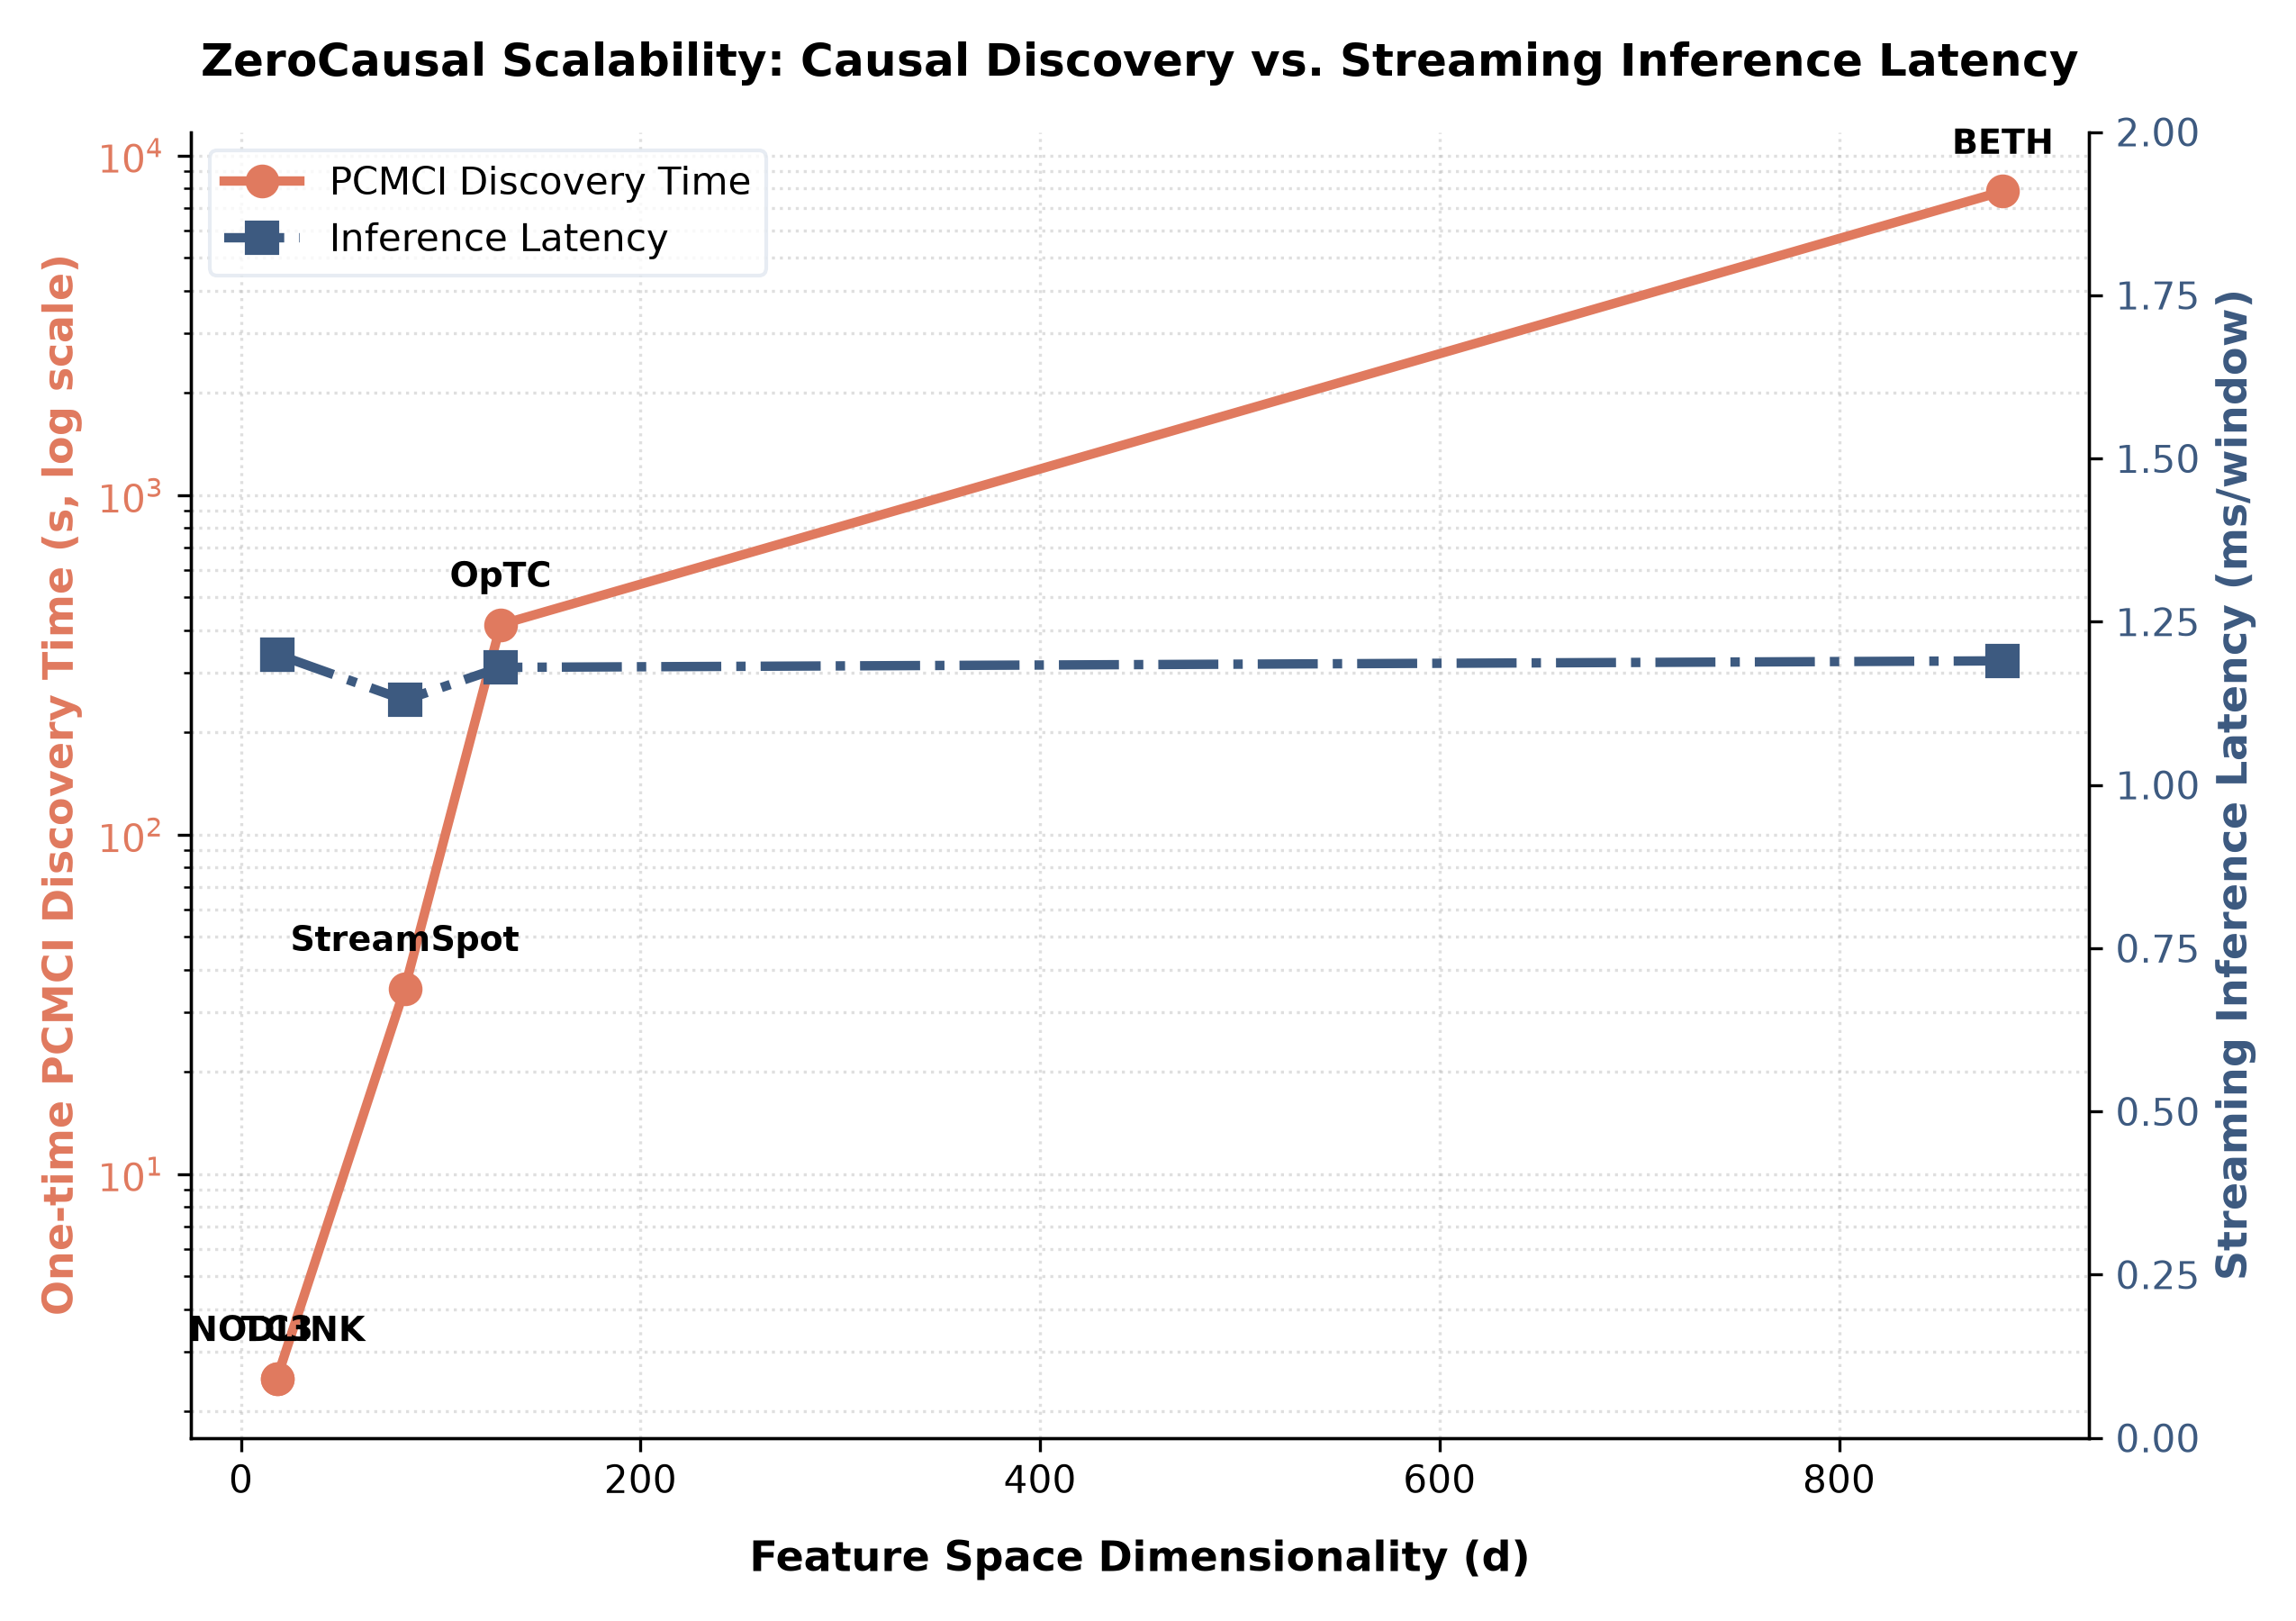
\includegraphics[width=\linewidth]{plots/dimensionality_vs_latency.png}}
\caption{Framework scalability: one-time offline PCMCI discovery time (log scale) and streaming inference latency (ms/window) vs. feature space dimensionality $d$.}
\label{fig:scalability_curve}
\end{figure}

\textit{Scaling to very high-dimensional feature spaces.}~For $d > 1000$ edge types (e.g., fine-grained kernel call logs), the PCMCI MCI test complexity grows approximately as $\mathcal{O}(d^2 \tau_{\max} T)$. Beyond $d \approx 1000$, a variance-thresholding or spectral feature selection pre-pass should be applied to reduce the effective dimension before discovery, as discussed in Section~\ref{sec:design}. At $d = 5000$ (extreme high-dimensional regime), the offline discovery time would project to $\approx$4--7 days on a CPU; GPU-accelerated robust covariance estimation (e.g., FastMCD) or distributed PCMCI can reduce this to under 6 hours and is a planned engineering extension.

\subsection{Causal Sufficiency}
We assume causal sufficiency---that no unobserved confounders jointly drive the observed provenance features. In enterprise networks, unobserved external variables (e.g., domain controller group-policy updates or NTP sync events) could induce statistical correlations that PCMCI falsely learns as direct causal edges, resulting in localized false alarms.
Our framework mitigates this through two mechanisms: (1) the conformal prediction layer calibrates alarm thresholds empirically on the observed fused score distribution, absorbing Type I error inflation, and (2) the change-point detector triggers periodic online refits, allowing spurious edges to be discarded when the distribution shifts.

\subsection{Linear Approximation on Sparse Streams}
The linear SCM variant generally matches or outperforms the non-linear Random Forest SCM on sparse, count-based provenance streams. This indicates that host audit logs behave approximately like linear aggregations of parent events. On zero-inflated data, non-linear regressors can overfit rare bursts and produce noisier residual rankings. The linear SCM serves as an efficient first-order mechanism approximation, while the non-linear regression option is retained for richer, continuous-valued event streams.

\subsection{StreamSpot: Analysis of Residual Weakness}
StreamSpot represents our most challenging benchmark (AUC 0.6909), and merits deeper analysis. The dataset contains 89,000 graphs from five heterogeneous workload types (YouTube, Gmail, VGame, Download, CNN), where each workload generates a qualitatively different causal graph structure. The key limitation is that a \emph{single} linear SCM learned from all five workload types is a poor fit for any individual type: the SCM equations are computed over a mixture distribution, producing systematically inflated residuals for workload-specific edge patterns, which in turn desensitizes the mechanism violation coordinates ($s_8$--$s_{11}$). The improvement from 0.4991 to 0.6909 comes primarily from the Temporal Reasoner ($R_T$) recognizing that a \emph{sequence} of states from an active drive-by download (elevated edge counts across multiple steps) differs from a normal workload transition (short transient spike). Two architectural improvements would significantly raise this number: (1) workload-type conditioning (fitting a separate SCM per identified workload cluster), and (2) mixture-of-experts SCMs that soft-assign each window to the nearest workload type. Both are targeted in our future work (Section~\ref{sec:future}).

\subsection{Threat Model Realization \& Mimicry Attacks}
We acknowledge a gap between our theoretical threat model (Section~\ref{sec:threat}) and experimental evaluations:
\begin{enumerate}
\item \textbf{SCM-Aware Mimicry}: If an attacker learns the system SCM's structure, they could attempt to orchestrate execution timings to mimic normal causal dependencies. However, successful mimicry requires satisfying all $d \times \tau_{\max}$ causal constraints in real time---a highly complex optimization challenge. Real APT campaigns naturally inject novel process-file edges with no causal parents in the baseline graph, triggering the structural novelty override ($s_{t,1}$) regardless of residual deviations. Empirical validation of active, SCM-aware mimicry attacks is left to future work.
\item \textbf{Calibration Poisoning}: Realized and evaluated through our contamination sweeps (Section~\ref{sec:eval_contamination}), demonstrating that RobustParCorr insulates causal structure learning up to 20\% contamination.
\item \textbf{Refit Blind Spots}: The adaptation window during SCM refitting represents a bounded-duration vulnerability ($\approx$1--2 conformal calibration cycles). Future work will explore transition-state alerting to cover this window.
\item \textbf{Stealthy Adaptive Attackers}: Evaluated through the multi-stage APT droppers in TC3 and OpTC. The temporal operator ($R_T$) successfully detects these via state sequence trajectory modeling.
\end{enumerate}

\subsection{Overcoming Operational Recall Barriers}
At a 95\% recall target, pure causal anomaly detectors exhibit an FPR of 44.57\% on OpTC and 96.40\% on StreamSpot. The Behavioral State Reasoning framework bridges this gap:
\begin{itemize}
\item On OpTC, the calibrated risk fusion layer reduces FPR at 95\% recall to \textbf{10.14\%} (a 4$\times$ false alarm reduction).
\item On StreamSpot, it reaches AUC \textbf{0.6909} (from 0.4991) and FPR at 95\% recall of \textbf{89.02\%}.
\end{itemize}
By utilizing conformal prediction, operators can set a fixed FPR budget (e.g., 5\%), and the system dynamically adjusts its alerting threshold within that budget.

\subsection{Ethical Considerations}
All datasets (DARPA OpTC, BETH, StreamSpot) are public or anonymized, containing no private user information. Our framework is designed strictly for defensive host monitoring.
